\begin{table}[t]
\centering\small
\caption{Realistic scenario (delays, missing and noisy outcomes, shocks, approval bias), 20 seeds, mean $\pm$ 95\% CI. Decision quality and transfer: nights 40--59, 0 = random choice, 1 = optimal. Headroom: share of the oracle's advantage over random retention. Rows above the rule are capacity-limited ($C=300$); keep everything is unbounded.}
\label{tab:main}
\begin{tabular}{@{}lccccr@{}}
\toprule
Policy & Decision quality $\uparrow$ & Transfer $\uparrow$ & ECE$^\ast$ $\downarrow$ & Regret (\%) $\downarrow$ & Headroom\\
\midrule
Random & 0.932{\scriptsize$\,\pm$0.014} & 0.912{\scriptsize$\,\pm$0.016} & 0.061{\scriptsize$\,\pm$0.007} & 19.0{\scriptsize$\,\pm$0.9} & 0\%\\
Random (resolved only) & 0.946{\scriptsize$\,\pm$0.010} & 0.921{\scriptsize$\,\pm$0.017} & 0.059{\scriptsize$\,\pm$0.006} & 14.8{\scriptsize$\,\pm$0.8} & 22\%\\
Recency (FIFO) & 0.927{\scriptsize$\,\pm$0.011} & 0.917{\scriptsize$\,\pm$0.016} & 0.058{\scriptsize$\,\pm$0.009} & 19.3{\scriptsize$\,\pm$1.1} & $<$0\%\\
Recurrence & 0.870{\scriptsize$\,\pm$0.018} & 0.822{\scriptsize$\,\pm$0.046} & 0.048{\scriptsize$\,\pm$0.005} & 29.8{\scriptsize$\,\pm$1.5} & $<$0\%\\
Similarity to recent queries & 0.902{\scriptsize$\,\pm$0.022} & 0.883{\scriptsize$\,\pm$0.023} & 0.043{\scriptsize$\,\pm$0.005} & 25.4{\scriptsize$\,\pm$2.2} & $<$0\%\\
Self-rated importance & 0.931{\scriptsize$\,\pm$0.013} & 0.920{\scriptsize$\,\pm$0.011} & 0.055{\scriptsize$\,\pm$0.009} & 19.3{\scriptsize$\,\pm$1.5} & $<$0\%\\
User preference (selection) & 0.921{\scriptsize$\,\pm$0.017} & 0.898{\scriptsize$\,\pm$0.026} & 0.050{\scriptsize$\,\pm$0.007} & 20.4{\scriptsize$\,\pm$1.3} & $<$0\%\\
User preference (as reward) & 0.370{\scriptsize$\,\pm$0.057} & 0.347{\scriptsize$\,\pm$0.037} & 0.386{\scriptsize$\,\pm$0.021} & 88.1{\scriptsize$\,\pm$2.0} & $<$0\%\\
Surprise (PER-style) & 0.935{\scriptsize$\,\pm$0.010} & 0.913{\scriptsize$\,\pm$0.016} & 0.115{\scriptsize$\,\pm$0.008} & 18.9{\scriptsize$\,\pm$1.6} & 4\%\\
Surprise (greedy top-$b$) & 0.498{\scriptsize$\,\pm$0.022} & 0.467{\scriptsize$\,\pm$0.024} & 0.132{\scriptsize$\,\pm$0.008} & 70.7{\scriptsize$\,\pm$1.4} & $<$0\%\\
\textbf{WHY} & \textbf{0.974{\scriptsize$\,\pm$0.004}} & \textbf{0.969{\scriptsize$\,\pm$0.004}} & 0.114{\scriptsize$\,\pm$0.005} & 13.3{\scriptsize$\,\pm$1.0} & 65\%\\
\midrule
Counterfactual oracle & 0.996{\scriptsize$\,\pm$0.001} & 0.993{\scriptsize$\,\pm$0.002} & 0.105{\scriptsize$\,\pm$0.021} & 13.8{\scriptsize$\,\pm$2.4} & 100\%\\
Keep everything (unbounded) & 0.993{\scriptsize$\,\pm$0.002} & 0.990{\scriptsize$\,\pm$0.003} & 0.077{\scriptsize$\,\pm$0.006} & 5.0{\scriptsize$\,\pm$0.4} & 95\%\\
\bottomrule
\end{tabular}
\end{table}


\begin{figure}[t]
\centering
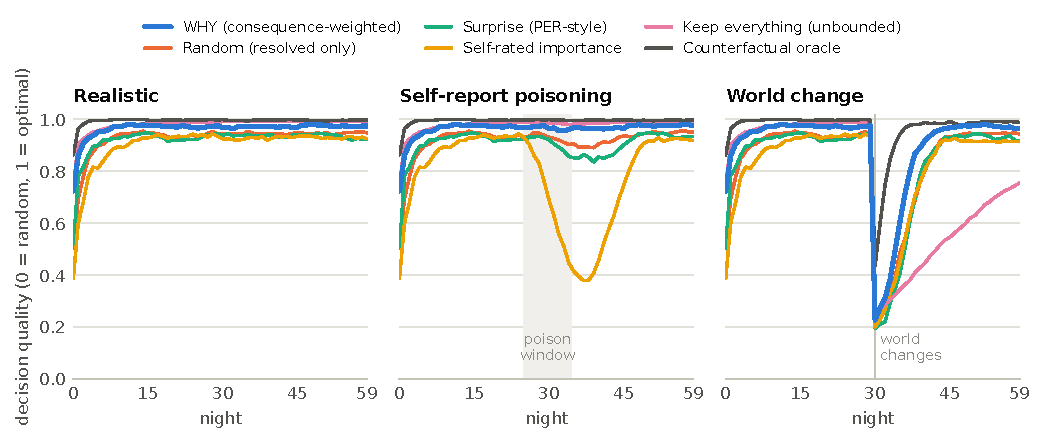
\includegraphics[width=\linewidth]{../figs/fig_curves.pdf}
\caption{Decision quality by night (mean of 20 seeds). Left: Realistic. Middle: a self-report poisoning campaign on days 25--34 (shaded). Right: two rule weights flip sign at night 30. Keep everything is unbounded; every other policy holds at most 300 episodes.}
\label{fig:curves}
\end{figure}

\subsection{Main comparison}
Table~\ref{tab:main} and Figure~\ref{fig:curves} (left) summarize the Realistic scenario. Consequence-weighted consolidation reached a late decision quality of \val{realistic-why-ndq_tr}\,$\pm$\,\val{realistic-why-ndq_tr-ci}, above every other capacity-limited policy. The strongest of those was random retention restricted to resolved outcomes (\val{realistic-random_resolved-ndq_tr}); WHY exceeded it by \val{pair-realistic-random_resolved-ndq_tr}\,$\pm$\,\val{pair-realistic-random_resolved-ndq_tr-ci} and was higher on \val{pair-realistic-random_resolved-ndq_tr-wins} of 20 seeds. Against the baselines named in the hypothesis, the paired differences were \val{pair-realistic-recency-ndq_tr} for recency, \val{pair-realistic-similarity-ndq_tr} for similarity, \val{pair-realistic-recurrence-ndq_tr} for recurrence, \val{pair-realistic-importance-ndq_tr} for self-rated importance, and \val{pair-realistic-user_pref-ndq_tr} for user preference, each positive on all 20 seeds. WHY captured \val{cap-realistic-why}\% of the oracle's headroom over random retention, compared with \val{cap-realistic-random_resolved}\% for the best competitor, and the gain carried over to held-out task families (transfer \val{realistic-why-ndq_ho} versus \val{realistic-random_resolved-ndq_ho}).

About \val{waitshare}\% of WHY's gain over plain random retention comes from waiting. Restricting random selection to resolved outcomes lifts decision quality from \val{realistic-random-ndq_tr} to \val{realistic-random_resolved-ndq_tr}, because a fifth of all outcomes never resolve and random retention fills about a fifth of its memory with episodes that will never carry a label (Table~\ref{tab:composition}). The rest comes from which resolved episodes the score selects.

Two references bracket the result. The counterfactual oracle reached \val{realistic-oracle-ndq_tr}. Unbounded memory reached \val{realistic-keep_all-ndq_tr} and beat WHY on every seed (paired difference \val{pair-realistic-keep_all-ndq_tr}): with 6{,}000 episodes and 13 parameters, label noise averages out and nothing needs to be forgotten. The hypothesis concerns capacity-limited memory; Section~\ref{sec:sweeps} shows how the comparison moves with capacity.

Two policies failed outright. Training on approval instead of outcomes (\val{realistic-user_pref_reward-ndq_tr}) learned that agreeable options succeed. Keeping the $b$ most surprising outcomes each night (\val{realistic-surprise_greedy-ndq_tr}) filled memory with corrupted and confounded labels; this is why the PER-style stochastic version is our main surprise baseline.

\begin{table}[t]
\centering\small
\caption{What each policy remembered: composition of durable memory (\% of engrams, 20 seeds). Categories are exclusive, assigned in the order shown. Realistic at night 59; poison share from the Poisoning scenario at night 34, the end of the attack.}
\label{tab:composition}
\setlength{\tabcolsep}{5pt}
\begin{tabular}{@{}lcccccc@{}}
\toprule
& \multicolumn{5}{c}{Realistic, night 59} & Poisoning\\
\cmidrule(lr){2-6}\cmidrule(lr){7-7}
Policy & \shortstack{Never\\resolves} & \shortstack{Shock-\\confounded} & \shortstack{Corrupted\\report} & \shortstack{Routine\\duplicate} & Other & \shortstack{Poison\\(night 34)}\\
\midrule
Random & 19.3 & 3.2 & 5.0 & 25.2 & 47.2 & 12.0\\
Recency (FIFO) & 19.6 & 4.0 & 5.0 & 24.8 & 46.6 & 10.7\\
Recurrence & 20.0 & 3.3 & 4.2 & 72.5 & 0.0 & 0.0\\
Similarity to recent queries & 20.3 & 3.0 & 4.7 & 27.1 & 45.0 & 10.4\\
Self-rated importance & 20.4 & 3.4 & 5.0 & 24.4 & 46.8 & 46.2\\
User preference (selection) & 19.4 & 3.0 & 5.1 & 25.3 & 47.2 & 17.4\\
Surprise (PER-style) & 0.0 & 5.3 & 8.1 & 31.2 & 55.3 & 11.7\\
\textbf{WHY} & 0.0 & 0.0 & 2.4 & 29.3 & 68.3 & 3.5\\
Counterfactual oracle & 0.0 & 0.8 & 1.4 & 32.8 & 65.1 & 3.4\\
\bottomrule
\end{tabular}
\end{table}


\subsection{What each policy remembered}
Table~\ref{tab:composition} shows the contents of durable memory. WHY's memory held no episodes that would never resolve and no shock-confounded outcomes, and corrupted self-reports fell from \val{comp-realistic-random-flip}\% under random retention to \val{comp-realistic-why-flip}\%. Recurrence-based consolidation kept nothing but routine duplicates (Table~\ref{tab:composition} counts some of them under earlier categories). PER-style surprise over-represented episodes that are surprising for the wrong reasons: corrupted reports (\val{comp-realistic-surprise-flip}\%) and shock-confounded outcomes (\val{comp-realistic-surprise-shock}\%).

\subsection{Misleading experiences}
Under the self-report poisoning campaign (Figure~\ref{fig:curves}, middle; Table~\ref{tab:scenarios}), self-rated importance lost \val{dmgabs-poison-importance} in decision quality over nights 25--44: poisoned episodes are maximally dramatic, the rater consolidated \val{pcons-poison-importance}\% of them (against \val{hcons-poison-importance}\% of honest episodes), and they made up \val{comp-poison-importance-poison}\% of its memory at the end of the attack. User preference lost \val{dmgabs-poison-user_pref}, PER-style surprise \val{dmgabs-poison-surprise}, and random retention \val{dmgabs-poison-random}. WHY lost \val{dmgabs-poison-why}; it consolidated \val{pcons-poison-why}\% of poisoned episodes against \val{hcons-poison-why}\% of honest ones, and poison made up \val{comp-poison-why-poison}\% of its memory, about the same as the oracle's \val{comp-poison-oracle-poison}\%. Unbounded memory also held up (it lost \val{dmgabs-poison-keep_all}), because 200 poisoned episodes were diluted by thousands of honest ones.

The protection comes from the channel discount, and it disappears when the channel lies. Without the discount, poison's share of WHY's memory grew \val{noM-poison-share-mult}-fold (Table~\ref{tab:ablation}). When the same false outcomes arrived as verified, WHY consolidated \val{pcons-poison_verified-why}\% of them, about \val{pratio-poison_verified-why} times its rate for honest episodes, poison reached \val{poison_verified-why-poison34}\% of its memory against \val{poison_verified-random-poison34}\% for random retention, and it lost \val{dmgabs-poison_verified-why} over nights 25--44, more than random retention (\val{dmgabs-poison_verified-random}). Two parts of the score favor poisoned outcomes once they pass verification: they are somewhat more surprising than the honest outcomes competing with them (mean surprise \val{check-vp-S-poison} versus \val{check-vp-S-honest} on nights 25--34), and the consequence factor favors same-day outcomes (Section~\ref{sec:ablations}).

Shocks are the other misleading experience, present in every Realistic run (\env{shockdays} shock days per run on average). The causal-confidence factor kept shock-confounded outcomes out of WHY's memory; removing it cost \val{ablabs-realistic-noK-ndq_tr} in decision quality.

\begin{table}[t]
\centering\small
\caption{Decision quality across scenarios (mean over 20 seeds; nights 40--59 unless noted). Poison damage: change in decision quality over nights 25--44 relative to the same policy in the Realistic scenario on identical base streams. World change: nights 30--39 (first ten nights after the change) and 50--59.}
\label{tab:scenarios}
\setlength{\tabcolsep}{4.5pt}
\begin{tabular}{@{}lccccccc@{}}
\toprule
& & & \multicolumn{2}{c}{Poison damage (25--44)} & \multicolumn{2}{c}{World change} \\
\cmidrule(lr){4-5}\cmidrule(lr){6-7}
Policy & Clean & Realistic & self-report & verified & 30--39 & 50--59\\
\midrule
Random & 0.971 & 0.932 & $-$0.039 & $-$0.039 & 0.459 & 0.921\\
Random (resolved only) & 0.971 & 0.946 & $-$0.027 & $-$0.027 & 0.454 & 0.945\\
Recency (FIFO) & 0.970 & 0.927 & $-$0.024 & $-$0.024 & 0.484 & 0.928\\
Recurrence & 0.913 & 0.870 & 0.000 & 0.000 & 0.363 & 0.854\\
Similarity to recent queries & 0.940 & 0.902 & $-$0.044 & $-$0.044 & 0.446 & 0.890\\
Self-rated importance & 0.965 & 0.931 & $-$0.331 & $-$0.331 & 0.448 & 0.915\\
User preference (selection) & 0.959 & 0.921 & $-$0.077 & $-$0.077 & 0.384 & 0.918\\
User preference (as reward) & 0.865 & 0.370 & $-$0.031 & $-$0.031 & 0.089 & 0.331\\
Surprise (PER-style) & 0.971 & 0.935 & $-$0.054 & $-$0.054 & 0.426 & 0.931\\
Surprise (greedy top-$b$) & 0.641 & 0.498 & $-$0.103 & $-$0.103 & 0.269 & 0.477\\
\textbf{WHY} & 0.977 & 0.974 & $-$0.004 & $-$0.060 & 0.557 & 0.972\\
\midrule
Counterfactual oracle & 0.997 & 0.996 & 0.000 & 0.000 & 0.838 & 0.990\\
Keep everything (unbounded) & 0.998 & 0.993 & $-$0.006 & $-$0.006 & 0.335 & 0.700\\
\bottomrule
\end{tabular}
\end{table}


\subsection{When the world changes}
Flipping two rule weights at night 30 (Figure~\ref{fig:curves}, right) turns old memories into misleading ones. Unbounded memory collapsed: its decision quality was \val{world_change-keep_all-ndq_post_early} over nights 30--39 and still \val{world_change-keep_all-ndq_post_late} over nights 50--59, because thirty days of pre-change evidence outvote the new world. Capacity-limited policies forget by construction and recovered. WHY recovered fastest among them (\val{world_change-why-ndq_post_early} over nights 30--39, against \val{world_change-recency-ndq_post_early} for recency and \val{world_change-random_resolved-ndq_post_early} for resolved-only random retention; the oracle reached \val{world_change-oracle-ndq_post_early}). This is the one scenario in which bounded memory beat unbounded memory; WHY's margin was \val{pair-world_change-keep_all-ndq_tr} in late decision quality. The causal-confidence factor slowed the first days of recovery: without it, WHY averaged \val{check-wc-noK-early} over nights 30--39 but \val{check-wc-noK-late} over nights 50--59 (full method: \val{check-wc-full-early} and \val{check-wc-full-late}), because a real change initially looks like a shock.

\subsection{Retroactive tagging}
Of the episodes WHY consolidated in the Realistic scenario, \val{retro-delayed}\% had outcomes that were still unresolved on the night they happened, against a base rate of \env{delayed}\% among resolvable outcomes and \val{retro-rr-delayed}\% for resolved-only random retention. Another \val{retro-rescored}\% had already resolved but were consolidated on a later night, after rescoring. The average engram was written \val{retro-lag} nights after the experience. Deciding once, on the first night, was the most damaging ablation in this scenario: it cost \val{ablabs-realistic-noretro-ndq_tr} in decision quality and was worse on all 20 seeds. Propagating tags from surprising outcomes to similar episodes added nothing measurable (\val{abl-realistic-prop-ndq_tr}). Section~\ref{sec:sweeps} shows that the value of deferral does not depend much on how many outcomes arrive late.
